\documentclass{article}

\usepackage{fancyhdr}
\usepackage{lastpage}
\usepackage{extramarks}
\usepackage[usenames,dvipsnames]{color}
\usepackage{amsmath}
\usepackage{amsthm}
\usepackage{amsfonts}
\usepackage{changepage}
\usepackage{lineno}
\usepackage[plain]{algorithm}
\usepackage{algpseudocode}
\usepackage{tikz}

\usetikzlibrary{arrows}
\usetikzlibrary{positioning}

\topmargin=-0.45in
\evensidemargin=0in
\oddsidemargin=0in
\textwidth=6.5in
\textheight=9.0in
\headsep=0.25in

\linespread{1.1}

\pagestyle{fancy}
\lhead{\hmwkAuthorName}
\chead{\hmwkClass\ (\hmwkClassInstructor\ \hmwkClassTime): \hmwkTitle}
\rhead{\firstxmark}
\lfoot{\lastxmark}
\cfoot{}

\renewcommand\headrulewidth{0.4pt}
\renewcommand\footrulewidth{0.4pt}

\setlength{\floatsep}{100pt}
\renewcommand{\algorithmicrequire}{\textbf{Input:}}
\renewcommand{\algorithmicensure}{\textbf{Output:}}

\setlength\parindent{0pt}

\newcommand{\enterProblemHeader}[1]{
    \nobreak\extramarks{}{Problem \arabic{#1} continued on next page\ldots}\nobreak{}
    \nobreak\extramarks{Problem \arabic{#1} (continued)}{Problem \arabic{#1} continued on next page\ldots}\nobreak{}
}

\newcommand{\exitProblemHeader}[1]{
    \nobreak\extramarks{Problem \arabic{#1} (continued)}{Problem \arabic{#1} continued on next page\ldots}\nobreak{}
    \stepcounter{#1}
    \nobreak\extramarks{Problem \arabic{#1}}{}\nobreak{}
}

\setcounter{secnumdepth}{0}
\newcounter{homeworkProblemCounter}
\setcounter{homeworkProblemCounter}{1}
\nobreak\extramarks{Problem \arabic{homeworkProblemCounter}}{}\nobreak{}

\newenvironment{homeworkProblem}{
    \section{Problem \arabic{homeworkProblemCounter}}
    \enterProblemHeader{homeworkProblemCounter}
}{
    \exitProblemHeader{homeworkProblemCounter}
}

\newcommand{\hmwkTitle}{Homework\ \#5}
\newcommand{\hmwkDueDate}{November 11, 2013 at 4:30pm}
\newcommand{\hmwkClass}{CS311}
\newcommand{\hmwkClassTime}{Section 3}
\newcommand{\hmwkClassInstructor}{Professor Lathrop}
\newcommand{\hmwkAuthorName}{Josh Davis}
\newcommand{\solution}{{\large \bfseries Solution}}

\title{
    \vspace{2in}
    \textmd{\textbf{\hmwkClass:\ \hmwkTitle}}\\
    \normalsize\vspace{0.1in}\small{Due\ on\ \hmwkDueDate}\\
    \vspace{0.1in}\large{\textit{\hmwkClassInstructor\ \hmwkClassTime}}
    \vspace{3in}
}

\author{\textbf{\hmwkAuthorName}}
\date{}

\newcommand{\alg}[1]{\textsc{\bfseries \footnotesize #1}}

\begin{document}

\maketitle

\pagebreak

\begin{homeworkProblem}
    Give algorithms for the following operations.
    \\

    \solution

    Algorithms for each part are below.
    \\

    \textbf{Part A}

    Give an algorithm that multiples two degree-1 polynomials with only three
    multiply operations.
    \\

    \begin{algorithm}[]
        \begin{algorithmic}[1]
            \Function{MultiplySingleDegreePolynomials}{$a, b, c, d$}
            \State{} \Return{$0$}
            \EndFunction{}
        \end{algorithmic}
        \caption{Multiply 1 degree polynomial}
    \end{algorithm}

    \textbf{Part B}

    Give a divide-and-conquer algorithm for multiplying two polynomials of degree \(n\). Prove
    using the master theorem that your algorithm runs in \(\Theta(n^{\log_2 3})\). You may assume
    that \(n + 1\) is a power of 2.
    \\

    \begin{algorithm}[]
        \begin{algorithmic}[1]
            \Function{MultiplyNDegreePolynomials}{}
            \State{} \Return{$0$}
            \EndFunction{}
        \end{algorithmic}
        \caption{Multiply \(n\) degree polynomial}
    \end{algorithm}
\end{homeworkProblem}

\pagebreak

\begin{homeworkProblem}
    Give an \(O(\log n)\) time algorithm that computes the following function:
    \\

    \alg{MEDIAN-OF-TWO($l_1, l_2$)}

    \begin{algorithm}[]
        \begin{algorithmic}[1]
            \Require \(l_1\) and \(l_2\) are two sorted lists of integers. Each
            list has \(n\) elements (\(2n\) elements in total) and the value of
            each element in the lists is unique.

            \Ensure The value of the \(n^{th}\) smallest integer in the set of
            \(2n\) integers is \(l_1\) and \(l_2\).
        \end{algorithmic}
    \end{algorithm}

    \solution

    \begin{algorithm}[]
        \begin{algorithmic}[1]
            \Function{Mid}{$x, y$}
                \State{} \Return{$(y - x) / 2 + x$}
            \EndFunction{}
            \\
            \Function{Median-Of-Two}{$l_1, l_2$}
                \State{} $start1 \gets 0$
                \State{} $start2 \gets 0$
                \State{} $end1 \gets l_1.length$
                \State{} $end2 \gets l_2.length$
                \State{} $mid1 \gets \Call{Mid}{start1, end1}$
                \State{} $mid2 \gets \Call{Mid}{start2, end2}$
                \\
                \While{$mid1 < end1$ and $mid2 < e2$}
                    \If{$l1[mid1] < l2[mid2]$}
                        \State{} $start1 \gets mid1$
                        \State{} $end2 \gets mid2$
                    \Else{}
                        \State{} $end1 \gets mid1$
                        \State{} $start2 \gets mid2$
                    \EndIf
                    \\
                    \State{} $mid1 \gets \Call{Mid}{start1, end1}$
                    \State{} $mid2 \gets \Call{Mid}{start2, end2}$
                \EndWhile
                \\
                \If{$mid1 \geq end1$}
                    \State{} \Return{$l1[mid1]$}
                \Else{}
                    \State{} \Return{$l2[mid2]$}
                \EndIf
            \EndFunction{}
        \end{algorithmic}
        \caption{Value of the \(n^{th}\) smallest integer in either list}
    \end{algorithm}
\end{homeworkProblem}

\pagebreak

\begin{homeworkProblem}
    Give an \(O(n)\) average case running time algorithm that computes the
    following:
    \\

    \alg{Kth-SMALLEST($list, k$)}

    \begin{algorithm}[]
        \begin{algorithmic}[1]
            \Require An unsorted list \(list\) of unique integers and an integer \(k\)

            \Ensure The value of the \(k^{th}\) smallest integer from the list
        \end{algorithmic}
    \end{algorithm}

    \solution

    The algorithm is based off of \alg{QuickSort} and is often called
    \alg{QuickSelect}.  The principle idea is to use the partitioning function
    of \alg{QuickSort} because the element that is selected to be a partition
    will be placed in its correct place in the list. The position then will tell
    us where to look for the \(k\)th item.

    \begin{algorithm}[]
        \begin{algorithmic}[1]
            \Function{Kth-SMALLEST}{$list, k$}
                \State{} $index \gets \Call{Kth-SMALLEST-REC}{list, k, 0, list.length}$
                \State{} \Return{$list[index]$}
            \EndFunction{}
            \\
            \Function{QuickSelect}{$list, k, start, end$}
                \If{$start >= end$}
                    \State{} \Return{$end$}
                \EndIf{}
                \\
                \State{} $partition \gets \Call{Partition}{list, k, start, end}$
                \\
                \If{$k < partition$}
                    \State{} \Return{} \Call{QuickSelect}{$list, start, partition - 1$}
                \ElsIf{$k > partition$}
                    \State{} \Return{} \Call{QuickSelect}{$list, partition + 1, end$}
                \EndIf{}
                \\
                \State{} \Return{$list[k]$}
            \EndFunction{}
        \end{algorithmic}
        \caption{Give the $k^{th}$ smallest integer from the list}
    \end{algorithm}

    Where the \alg{Partition} algorithm is dependent on the type of
    partitioning scheme used.
\end{homeworkProblem}

\pagebreak

\begin{homeworkProblem}
    Let \(T\) be a tree with \(n\) vertices. We say that a vertex \(v\) is a
    \texttt{minimal separator of T} if its removal splits \(T\) into
    two or more subtrees, each with at most \(n/2\) nodes.
    \\

    \solution
    \\

    \textbf{Part A}

    Show that ever finite tree has at least one minimal separator.

    \begin{proof}

    \end{proof}

    \textbf{Part B}

    Show an \(O(\left\vert{V}\right\vert)\) algorithm for identifying a minimal
    separator in a given tree.

    \begin{algorithm}[]
        \begin{algorithmic}[1]
            \Function{MinimalSeparator}{$T$}
            \State{} \Return{$0$}
            \EndFunction{}
        \end{algorithmic}
        \caption{Identify a minimal separator in the given tree}
    \end{algorithm}

\end{homeworkProblem}

\pagebreak

\begin{homeworkProblem}
    Give an algorithm that computes the following:
    \\

    \alg{BST-Reconstruction($traversal$)}

    \begin{algorithm}[]
        \begin{algorithmic}[1]
            \Require An array of elements generated by a pre-order traversal of
            some binary search tree.

            \Ensure A binary search tree identical to the original tree.
        \end{algorithmic}
    \end{algorithm}

    \solution

    Solution for the function is below:

    \begin{algorithm}[]
        \begin{algorithmic}[1]
            \Function{BST-Reconstruction}{$traversal$}
            \State{} \Return{$0$}
            \EndFunction{}
        \end{algorithmic}
        \caption{Binary search tree reconstruction}
    \end{algorithm}
\end{homeworkProblem}

\pagebreak

\begin{homeworkProblem}
    Let \(G = (V, E)\) be a connected, undirected graph.
    \\

    Prove or disprove:
    \[
        \exists v \in V \mid G = (V \setminus \{ v \}, E) \mbox{ is connected }
    \]

    \solution

\end{homeworkProblem}

\pagebreak

\begin{homeworkProblem}
    A \textit{mother} vertex in a directed graph \(G = (V, E)\) is a vertex \(v\)
    such that all other vertices in \(G\) can be reached by a directed path from \(v\).
    \\

    \solution
    \\

    \textbf{Part A}

    Give an \(O(n + m)\) algorithm to test whether a given vertex \(v\) is a
    mother of \(G\), where \(n = \left\vert V \right\vert\) and \(m =
    \left\vert E \right\vert\).
    \\

    \begin{algorithm}[]
        \begin{algorithmic}[1]
            \Function{IsMother}{$v, G$}
            \State{} \Return{$0$}
            \EndFunction{}
        \end{algorithmic}
        \caption{Determine if a given vertex is a mother of a graph}
    \end{algorithm}

    \textbf{Part B}

    Give an \(O(n + m)\) algorithm to test whether a graph \(G\) contains a
    mother vertex.

    \begin{algorithm}[]
        \begin{algorithmic}[1]
            \Function{ContainsAMother}{$G$}
            \State{} \Return{$0$}
            \EndFunction{}
        \end{algorithmic}
        \caption{Determine if a given graph has a mother}
    \end{algorithm}
\end{homeworkProblem}

\pagebreak

\begin{homeworkProblem}
    Suppose we are given the minimum spanning tree \(T\) of a given graph \(G\)
    and a new edge \(e = (u, v)\) of weight \(w\) that we will add to \(G\).
    \\

    \solution

    Give an \(O(n)\) algorithm to find the minimum spanning tree of the graph
    \(G + e\).

    \begin{algorithm}[]
        \begin{algorithmic}[1]
            \Function{AddMST}{$T, e, G$}
            \State{} \Return{$0$}
            \EndFunction{}
        \end{algorithmic}
        \caption{Add an edge to a given minimum spanning tree}
    \end{algorithm}
\end{homeworkProblem}

\pagebreak

\begin{homeworkProblem}
    Problem 6--7 from the text.
    \\

    \solution
    \\

    \textbf{Part A}

    Let \(T\) be a minimum spanning tree of a weighted graph \(G\). Construct a
    new graph \(G'\) by adding a weight of \(k\) to every edge of \(G\). Do the
    edges of \(T\) form a minimum spanning tree of \(G'\)? Prove the statement
    or give a counterexample.

    \begin{proof}

    \end{proof}

    \textbf{Part B}

    Let \(P = \{s, \ldots, t \}\) describe the shortest weighted path between
    vertices \(s\) and \(t\) of a weighted graph \(G\). Construct a new graph
    \(G'\) by adding a weight of \(k\) to every edge of \(G\). Does \(P\)
    describe a shortest path from \(s\) to \(t\) in \(G'\)? Prove the statement
    or give a counterexample.
    \\

    \textbf{Counterexample}

    \(P\) still does not necessarily describe a shortest path from \(s\) to
    \(t\) in \(G'\).  This is weight added to each path is dependent on how
    many sections are in the path. If we were to let \(k = 5\) and add it to
    each path, a path that has 1 edge will have 5 added to it, but a path with
    2 edges will get 10 added to it. This is illustrated in the below example.
    \\

    The first figure, Figure~\ref{fig:graph1} is \(G\) and that path is the
    three edges straight across the line of nodes, from \(s\) to \(t\) then to
    \(u\). However the second graph is Figure~\ref{fig:graph2} has had \(k\)
    added to each edge, the shortest path is now the single edge from \(s\) to
    \(u\).
    \\

    \begin{figure}[h]
        \centering
        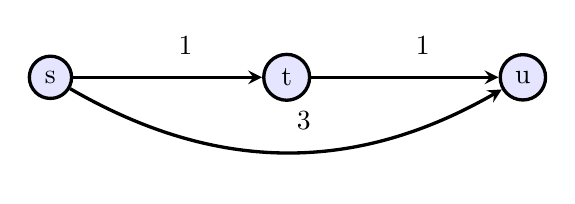
\begin{tikzpicture}[->,>=stealth,node distance=3cm,very
            thick,node/.style={circle,fill=blue!10,draw}]

            \node[node] (s) {s};
            \node[node] (t) [right of=s] {t};
            \node[node] (u) [right of=t] {u};

            \path[every node]

            (s) edge node [above=4mm, right] {1} (t)
                edge [bend right] node [above=4mm, right] {3} (u)
            (t) edge node [above=4mm, right] {1} (u);
        \end{tikzpicture}
        \caption{The graph \(G\).}
        \label{fig:graph1}

        \vspace{.2in}

        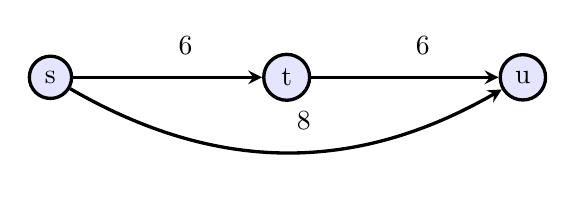
\begin{tikzpicture}[->,>=stealth,node distance=3cm,very
            thick,node/.style={circle,fill=blue!10,draw}]

            \node[node] (s) {s};
            \node[node] (t) [right of=s] {t};
            \node[node] (u) [right of=t] {u};

            \path[every node]

            (s) edge node [above=4mm, right] {6} (t)
                edge [bend right] node [above=4mm, right] {8} (u)
            (t) edge node [above=4mm, right] {6} (u);
        \end{tikzpicture}
        \caption{The graph \(G'\).}
        \label{fig:graph2}
    \end{figure}

\end{homeworkProblem}

\end{document}
